% ============================================================================
% ARTORYX --- MASTER DEVELOPMENT & PAYMENT AGREEMENT
% Copy retained by: ArtoryX (Developer)
% Compile with: pdflatex Agreement_ArtoryX_Copy.tex
% ============================================================================
\documentclass[a4paper, 11pt]{article}

% --- Page Geometry ---
\usepackage[
  top=20mm, bottom=18mm, left=24mm, right=24mm,
  headheight=14pt
]{geometry}

% --- Fonts ---
\usepackage[utf8]{inputenc}
\usepackage[T1]{fontenc}
\usepackage[scaled=0.95]{helvet}
\usepackage{inconsolata}
\renewcommand{\familydefault}{\sfdefault}

% --- Packages ---
\usepackage[dvipsnames]{xcolor}
\usepackage{titlesec}
\usepackage{fancyhdr}
\usepackage{enumitem}
\usepackage{tabularx}
\usepackage{graphicx}
\usepackage{tikz}
\usepackage{parskip}
\usepackage{microtype}
\usepackage{hyperref}
\usepackage{lastpage}
\usepackage{amssymb}
\usepackage{colortbl}
\usepackage{array}
\usepackage{calc}

% --- Color Palette ---
\definecolor{brand}{HTML}{111827}
\definecolor{accent}{HTML}{1E3A5F}
\definecolor{accentlight}{HTML}{EBF0F7}
\definecolor{muted}{HTML}{6B7280}
\definecolor{lightgray}{HTML}{F8F9FA}
\definecolor{bordergray}{HTML}{E5E7EB}
\definecolor{divider}{HTML}{D1D5DB}
\definecolor{gold}{HTML}{B8860B}
\definecolor{darkblue}{HTML}{0F172A}

% --- Hyperref Setup ---
\hypersetup{
  colorlinks=false,
  pdfauthor={ArtoryX},
  pdftitle={Master Development and Payment Agreement},
  pdfborder={0 0 0},
}

% --- Header / Footer ---
\pagestyle{fancy}
\fancyhf{}
\renewcommand{\headrulewidth}{0pt}
\renewcommand{\footrulewidth}{0pt}
\fancyfoot[L]{%
  
\begin{tikzpicture}[baseline=(current bounding box.center)]
    \fill[brand] (0,0) rectangle (2pt, 8pt);
    \node[anchor=west, inner sep=0pt] at (6pt, 4pt) {%
      \footnotesize\color{muted}\textsf{ArtoryX \;\textbar\; Confidential}%
    };
  \end{tikzpicture}%
}
\fancyfoot[R]{\footnotesize\color{muted}\textsf{\thepage\;/\;\pageref{LastPage}}}
\fancyhead[R]{%
  \footnotesize\color{muted}\textsf{Copy retained by: ArtoryX (Developer)}%
}

% --- First page style ---
\fancypagestyle{firstpage}{%
  \fancyhf{}
  \renewcommand{\headrulewidth}{0pt}
  \fancyfoot[L]{%
    
\begin{tikzpicture}[baseline=(current bounding box.center)]
      \fill[brand] (0,0) rectangle (2pt, 8pt);
      \node[anchor=west, inner sep=0pt] at (6pt, 4pt) {%
        \footnotesize\color{muted}\textsf{ArtoryX \;\textbar\; Confidential}%
      };
    \end{tikzpicture}%
  }
  \fancyfoot[R]{\footnotesize\color{muted}\textsf{\thepage\;/\;\pageref{LastPage}}}
}

% --- Section Styling ---
\titleformat{\section}
  {\normalsize\bfseries\color{brand}\sffamily\MakeUppercase}
  {}
  {0em}
  {\tikz[baseline=(char.base)]{
    \node[fill=brand, text=white, inner xsep=6pt, inner ysep=2.5pt, font=\footnotesize\bfseries] (char) {SECTION \thesection};
  }\;\;}
\titlespacing*{\section}{0pt}{14pt}{5pt}

\titleformat{\subsection}
  {\small\bfseries\color{accent}}
  {\thesubsection}
  {0.5em}
  {}
\titlespacing*{\subsection}{0pt}{7pt}{2pt}

% --- Custom Commands ---
\newcommand{\sectionrule}{%
  {\color{bordergray}\hrule height 0.4pt}%
  \vspace{5pt}%
}

\newcommand{\blankfield}[1]{%
  {\color{divider}\leaders\hrule height -1pt depth 1.6pt\hskip #1\relax}%
}

\newcommand{\statusbadge}[1]{%
  \tikz[baseline=(char.base)]{
    \node[fill=brand, text=white, inner xsep=5pt, inner ysep=1.5pt,
          rounded corners=2pt, font=\scriptsize\bfseries\sffamily] (char) {#1};
  }%
}

\newcommand{\clausenum}[1]{%
  {\color{accent}\textbf{#1}}\;%
}

% --- List Styling ---
\setlist[enumerate,1]{label=\color{accent}\textbf{(\alph*)}, leftmargin=2em, itemsep=1.5pt, parsep=0pt, topsep=2pt}
\setlist[itemize,1]{label=\color{accent}{\small$\blacktriangleright$}, leftmargin=1.5em, itemsep=1pt, parsep=0pt}

% --- Paragraph Spacing ---
\setlength{\parskip}{3.5pt}
\setlength{\parindent}{0pt}

% ============================================================================
\begin{document}
\thispagestyle{firstpage}

% === TITLE BLOCK ===
\begin{tikzpicture}[remember picture, overlay]
  % Dark header
  \fill[brand] (current page.north west) rectangle
    ([yshift=-52mm]current page.north east);
  % Gold accent line
  \fill[gold] ([yshift=-52mm]current page.north west) rectangle
    ([yshift=-52.8mm]current page.north east);
\end{tikzpicture}

\vspace*{-14mm}

\begin{center}
  {\color{white!50}\footnotesize\sffamilyCOPY RETAINED BY: ARTORYX (DEVELOPER)}\\[12pt]
  {\color{white}\fontsize{30}{34}\selectfont\textbf{\textsf{ARTORYX}}}\\[5pt]
  {\color{white!80}\small\sffamilyMASTER DEVELOPMENT \& PAYMENT AGREEMENT}\\[8pt]
  {\color{gold}\rule{50mm}{0.6pt}}\\[8pt]
  {\color{white!70}\footnotesize\sffamily
    Project: Daichiro Professional Skills Academy --- Full-Stack Web Application\\[2pt]
    Domain: \texttt{daichiro.in}%
  }
\end{center}

\vspace{10mm}

% === PARTIES BOX ===
\noindent
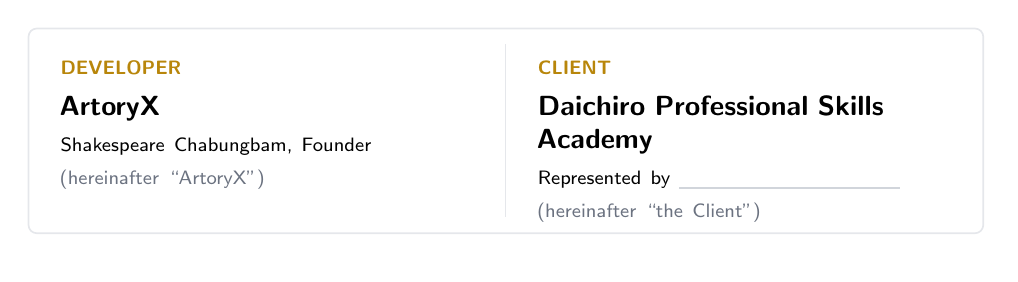
\begin{tikzpicture}
  % Outer border
  \draw[bordergray, line width=0.6pt, rounded corners=3pt]
    (0,0) rectangle (\textwidth, -26mm);
  % Center divider
  \draw[bordergray, line width=0.4pt]
    (0.5\textwidth, -2mm) -- (0.5\textwidth, -24mm);
  % Left party
  \node[anchor=north west, text width=0.44\textwidth, inner sep=4mm] at (0,0) {
    {\scriptsize\color{gold}\textbf{DEVELOPER}}\\[3pt]
    {\normalsize\textbf{ArtoryX}}\\[1pt]
    {\scriptsize Shakespeare Chabungbam, Founder}\\
    {\scriptsize\color{muted}(hereinafter ``ArtoryX'')}
  };
  % Right party
  \node[anchor=north west, text width=0.44\textwidth, inner sep=4mm] at (0.5\textwidth,0) {
    {\scriptsize\color{gold}\textbf{CLIENT}}\\[3pt]
    {\normalsize\textbf{Daichiro Professional Skills Academy}}\\[1pt]
    {\scriptsize Represented by \blankfield{28mm}}\\
    {\scriptsize\color{muted}(hereinafter ``the Client'')}
  };
\end{tikzpicture}

\vspace{2mm}
{\small\color{muted} Date of Agreement:\; \blankfield{35mm}}

\vspace{1mm}
{\small Both parties agree to the following terms and conditions.}

% =========================================
\section{Scope of Work}
\sectionrule

\subsection{Technology Stack}
\vspace{-2pt}
{\small
\begin{tabularx}{\textwidth}{@{}>{\color{accent}\bfseries}l @{\hspace{8pt}} X@{}}
  Frontend  & HTML, CSS, JavaScript \\
  Backend   & Python, Flask \\
  Database  & PostgreSQL \\
  AI Engine & Google Gemini AI (Vision + Text Generation) \\
  Server    & AWS EC2 (Ubuntu), Nginx, Gunicorn \\
\end{tabularx}}

\subsection{Deliverables}
\vspace{-2pt}
{\small
\begin{enumerate}
  \item Full-stack web application deployed at \texttt{daichiro.in}
  \item Public website --- Booking, About, SkillNest, Sunday Programs
  \item Admin Dashboard
  \item Employee Staff Portal (role-based, permission-controlled)
  \item Client Assessment Portal (self-destructing credentials)
  \item AWS EC2 deployment with Gunicorn + systemd
  \item Nginx reverse proxy with HTTPS / SSL
  \item PostgreSQL database schema and backup scripts
  \item Sitemap, robots.txt, SEO structure
  \item Maintenance page for downtime
\end{enumerate}}

\subsection{Features}
\vspace{-2pt}
{\small
\begin{enumerate}
  \item Appointment Booking --- Phone validation, package selection, price-locking, open/close control
  \item AI Career Assessment (5-Step) --- Auto-save, Gemini AI analysis, PDF reports, OCR scan via Gemini Vision
  \item SkillNest Admissions --- Seat cap, open/close toggle, admin workflow
  \item Invoice \& Email --- HTML invoice emails via Gmail SMTP, password reset with signed tokens
  \item Employee Permissions --- Granular role-based access control
  \item Admin Panel --- Full control over all data and settings
  \item Site Config Store --- All settings manageable from admin panel
  \item Background Automation --- Client auto-expiry (3 hrs), archival (90 days)
  \item Security --- CSRF, rate limiting, HSTS, CSP, XSS headers, bcrypt, secure sessions
  \item Developer Credit Portal --- ArtoryX's branded credit management
\end{enumerate}}


% =========================================
\section{Payment Milestones}
\sectionrule

{\small
\clausenum{2.1} All payments are non-refundable. Both phases are now complete.

\clausenum{2.2} Total Project Fee: Rs.\;\blankfield{25mm}\; (Rupees \blankfield{45mm}).

\vspace{3mm}
\noindent
\begin{tabularx}{\textwidth}{@{} >{\bfseries\small}l | >{\small\arraybackslash}X | >{\small\arraybackslash}X @{}}
  \arrayrulecolor{bordergray}
  \hline
  \rowcolor{accentlight}
  & \textbf{Phase 1 --- Advance} & \textbf{Phase 2 --- Final} \\
  \hline
  Amount   & Rs. 9,000 (Nine Thousand Only) & Rs.\;\blankfield{22mm} \\
  Received & 24 March 2025                  & 22 May 2025 \\
  Method   & Google Pay (UPI)               & \blankfield{22mm} \\
  Status   & \statusbadge{RECEIVED}         & \statusbadge{RECEIVED} \\
  \hline
\end{tabularx}
}


% =========================================
\section{Maintenance \& Support}
\sectionrule

{\small
\clausenum{3.1}\textbf{Warranty:}
Starting from the date of this Agreement, ArtoryX provides a 14-day warranty to fix critical bugs in the delivered code. This does not cover issues caused by third-party modifications, server changes, or Client interference.

\clausenum{3.2}\textbf{Maintenance Fees (Prepaid):}
All maintenance fees must be paid in advance before each billing period. Services will not commence until payment is received.

\vspace{2mm}
\noindent
\begin{tabularx}{\textwidth}{@{} >{\bfseries\small\color{accent}}l @{\hspace{8pt}} >{\small}X @{}}
  \arrayrulecolor{bordergray}
  Complimentary & First 1 month from final payment --- included at no charge. \\[4pt]
  Phase A       & Next 6 months --- Rs. 2,000/month, prepaid monthly (Total: Rs. 12,000). Covers monitoring, bug fixes, minor updates, and support. \\[4pt]
  Phase B       & After Phase A onwards (select one):\\
                & \;$\square$\; Option 1: Rs. 1,500/month, prepaid monthly\\
                & \;$\square$\; Option 2: Rs. 4,800/quarter, prepaid quarterly\\
\end{tabularx}

\vspace{2mm}
\clausenum{3.3}\textbf{Non-Payment:}
If prepayment is not received before the billing period begins, services will not be provided. ArtoryX is not responsible for any issues during unpaid periods.

\clausenum{3.4}\textbf{Out-of-Scope Work:}
New features, major redesigns, database restructuring, or server migration are not included. These will be quoted and billed separately.
}


% =========================================
\section{AWS Hosting \& Liability}
\sectionrule

{\small
\clausenum{4.1} The application runs on AWS EC2 (Mumbai Region) with Nginx and Gunicorn.

\clausenum{4.2} The Client is solely responsible for their AWS account --- including EC2, databases, storage, DNS, billing, and all associated services.

\clausenum{4.3} ArtoryX has delivered deployment-ready code. ArtoryX bears no liability for the Client's production environment --- including server crashes, security breaches, data loss, downtime, or AWS billing.
}


% =========================================
\section{Code Integrity \& Warranty Void}
\sectionrule

{\small
\clausenum{5.1} If the Client, any third-party developer, or any unauthorised person modifies the server environment, database, or deployment configuration --- all risk transfers to the Client immediately.

\clausenum{5.2} Repair work caused by unauthorised changes voids all warranties and will be invoiced separately as emergency repair.
}


% =========================================
\section{Confidentiality}
\sectionrule

{\small
\clausenum{6.1} ArtoryX will not share, sell, or disclose any Client data --- including student records, assessment data, credentials, or business information.

\clausenum{6.2} Both parties agree to keep all project discussions, pricing, and business assets confidential during and after this Agreement.

\clausenum{6.3}\textbf{Breach by ArtoryX:}
If ArtoryX is found to have disclosed, shared, or misused any confidential Client data in violation of this Section, the Client shall have the right to pursue legal action against ArtoryX. ArtoryX shall be held fully liable for any damages resulting from such breach.

\clausenum{6.4} This obligation survives for 3 years after termination of this Agreement.
}


% =========================================
\section{Ownership \& Intellectual Property}
\sectionrule

{\small
\clausenum{7.1} ArtoryX retains ownership of the source code, database schemas, deployment scripts, and all configuration files. The application has been deployed and is fully operational on the Client's server.

\clausenum{7.2}\textbf{Source Code Availability:}
The source code has not been handed over to the Client at this time. The Client may request a copy by providing written notice to ArtoryX. Delivery shall be subject to the terms in Section 9.6.

\clausenum{7.3} ArtoryX retains the right to use the project's visual design in its portfolio and marketing materials.
}


% =========================================
\section{Cancellation \& Refund Policy}
\sectionrule

{\small
\clausenum{8.1} The project has been completed and fully paid. All payments received by ArtoryX are final.

\clausenum{8.2} The Client may cancel maintenance with 30 days written notice. No refunds for the current billing cycle.
}


% =========================================
\section{Acceptance \& Testing}
\sectionrule

{\small
\clausenum{9.1} ArtoryX has provided the completed application for the Client's review and testing.

\clausenum{9.2} The Client has 7 days from the date of this Agreement to test and report defects in writing.

\clausenum{9.3} If no defects are reported within 7 days, the application is deemed accepted and meets all agreed specifications.

\clausenum{9.4} Only defects that deviate from the agreed scope (Section 1) qualify for free correction. New features or design preferences are out-of-scope (Section 3.4).

\clausenum{9.5} After acceptance, issues are governed by the Warranty (Section 3.1) and Maintenance terms (Section 3.2) only.

\clausenum{9.6}\textbf{Source Code Handover \& Agreement Termination:}
If the Client requests the source code (Section 7.2), or if any issue cannot be resolved through Warranty or Maintenance, ArtoryX shall provide the complete source code, database schemas, deployment scripts, and all files needed to independently operate the application.

Upon source code delivery, this Agreement is immediately and permanently terminated:
\begin{enumerate}
  \item The Client assumes full and exclusive responsibility for the application, its operation, and all associated risks;
  \item All of ArtoryX's obligations --- including warranty, maintenance, support, and liability --- are permanently ended;
  \item ArtoryX bears absolutely no risk, responsibility, or liability of any kind related to this website;
  \item No claims of any nature may be made against ArtoryX after source code delivery.
\end{enumerate}
}


% =========================================
\section{Disclaimer of Warranties}
\sectionrule

{\small
\clausenum{10.1} After the 14-day Warranty Period, the application is provided ``AS IS''.

\clausenum{10.2} ArtoryX does not guarantee uninterrupted operation, as the application depends on external factors (server uptime, network, third-party APIs).

\clausenum{10.3} Third-party services (Google Gemini AI, OCR, automated reports) are operated by their respective providers. ArtoryX is not responsible for their accuracy, reliability, or future compatibility.

\clausenum{10.4} ArtoryX has delivered a professionally engineered application built to current industry standards.

\clausenum{10.5} ArtoryX bears no liability for failures, pricing changes, deprecation, or discontinuation of third-party services (Google Gemini AI, AWS, Gmail SMTP, open-source libraries).
}


% =========================================
\section{Client Responsibilities}
\sectionrule

{\small
The Client is responsible for:
\begin{enumerate}
  \item Testing the application during the 7-day Acceptance Period and 14-day Warranty Period, and reporting issues in writing within those timeframes.
  \item Having provided accurate and timely information during development. ArtoryX is not responsible for issues caused by incomplete or delayed input.
  \item Ensuring their use of the application complies with all applicable laws, including data protection and privacy regulations.
\end{enumerate}
}


% =========================================
\section{Limitation of Liability}
\sectionrule

{\small
\clausenum{12.1} ArtoryX's maximum total liability under this Agreement shall not exceed the total fees received from the Client.

\clausenum{12.2} ArtoryX is not liable for:
\begin{enumerate}
  \item Indirect, incidental, consequential, or punitive damages;
  \item Loss of revenue, profit, or business;
  \item Loss of data or data corruption;
  \item Business interruption or downtime;
  \item Damages from the Client's failure to maintain backups or security.
\end{enumerate}
}


% =========================================
\section{Force Majeure}
\sectionrule

{\small
Neither party is liable for failures caused by events beyond reasonable control --- including natural disasters, pandemics, government actions, war, power failures, or internet outages.
}


% =========================================
\section{Dispute Resolution}
\sectionrule

{\small
\clausenum{14.1} This Agreement is governed by the laws of India.

\clausenum{14.2} Disputes shall first be resolved through good-faith negotiation within 30 days.

\clausenum{14.3} If unresolved, disputes shall be subject to the exclusive jurisdiction of the courts at Imphal, Manipur, India.
}


% =========================================
\section{General Provisions}
\sectionrule

{\small
\clausenum{15.1} This Agreement constitutes the entire understanding between both parties and supersedes all prior agreements, written or oral.

\clausenum{15.2} Amendments require written consent signed by both parties.

\clausenum{15.3} If any provision is found invalid, the remaining provisions remain in full effect.

\clausenum{15.4} ArtoryX is an independent contractor. This Agreement does not create a partnership, joint venture, or employment relationship.
}

\vspace{8mm}

% =========================================
% SIGNATURES
% =========================================
\noindent

\begin{tikzpicture}
  \fill[brand] (0,0) rectangle (\textwidth, -4mm);
\end{tikzpicture}

\vspace{4mm}
\begin{center}
  {\large\bfseries\color{brand}\sffamilySIGNATURES}
\end{center}
\vspace{1mm}

{\small\color{muted}
By signing below, both parties confirm they have read, understood, and agree to all terms in this Agreement.
}

\vspace{6mm}

\noindent
\begin{minipage}[t]{0.46\textwidth}
  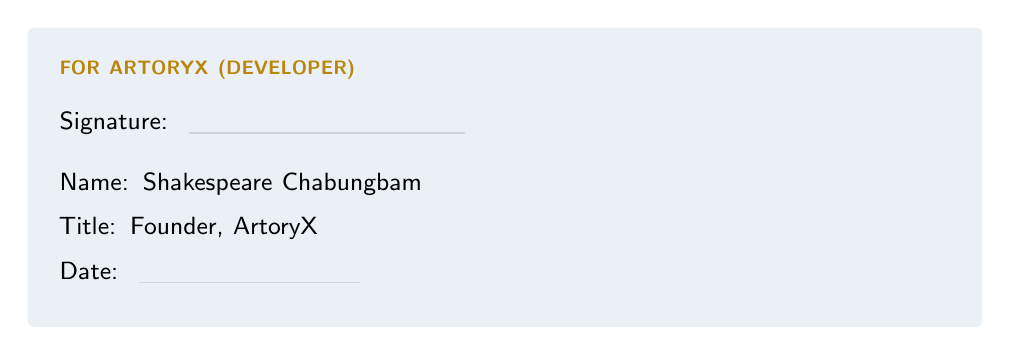
\begin{tikzpicture}
    \fill[accentlight, rounded corners=2pt] (0,0) rectangle (\textwidth, -38mm);
    \node[anchor=north west, text width=\textwidth-8mm, inner sep=4mm] at (0,0) {
      {\scriptsize\color{gold}\textbf{FOR ARTORYX (DEVELOPER)}}\\[8pt]
      {\small Signature:\; \blankfield{35mm}}\\[10pt]
      {\small Name: Shakespeare Chabungbam}\\[4pt]
      {\small Title: Founder, ArtoryX}\\[4pt]
      {\small Date:\; \blankfield{28mm}}
    };
  \end{tikzpicture}
\end{minipage}
\hfill
\begin{minipage}[t]{0.46\textwidth}
  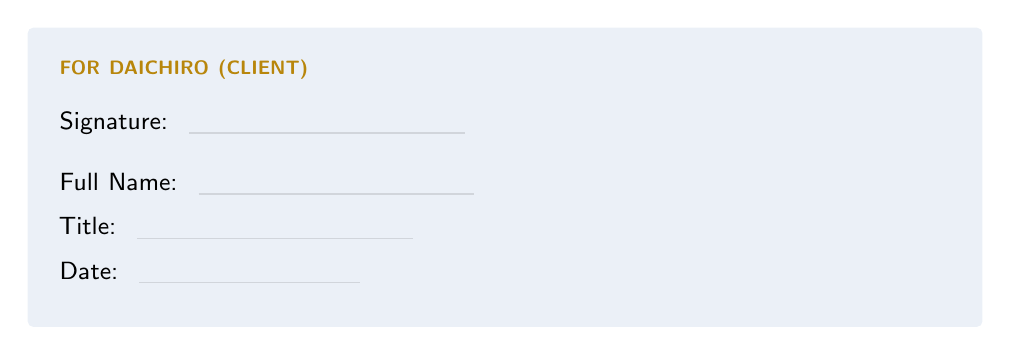
\begin{tikzpicture}
    \fill[accentlight, rounded corners=2pt] (0,0) rectangle (\textwidth, -38mm);
    \node[anchor=north west, text width=\textwidth-8mm, inner sep=4mm] at (0,0) {
      {\scriptsize\color{gold}\textbf{FOR DAICHIRO (CLIENT)}}\\[8pt]
      {\small Signature:\; \blankfield{35mm}}\\[10pt]
      {\small Full Name:\; \blankfield{35mm}}\\[4pt]
      {\small Title:\; \blankfield{35mm}}\\[4pt]
      {\small Date:\; \blankfield{28mm}}
    };
  \end{tikzpicture}
\end{minipage}

\vspace{8mm}
\begin{center}
  {\color{gold}\rule{40mm}{0.5pt}}\\[4pt]
  {\footnotesize\color{muted}END OF AGREEMENT}
\end{center}

\end{document}
